\chapter{General method}\label{chapter03}

The studies of this book share parts of their methodology: That is, the production study (Chapter \ref{chapter04}), the linear discriminative learning implementation (Chapter \ref{chapter05}), the perception study (Chapter \ref{chapter06}), and the comprehension study on plural and clitic /s/ (Chapter \ref{chapter08}) all make use of the same set of pseudowords. Pseudowords as a type of item are described in Section \ref{section03_1_1}, before Section \ref{section03_1_2} explains how the pertinent pseudowords were created. The perception study (Chapter \ref{chapter06}) and the comprehension study on non-morphemic and plural /s/ (Chapter \ref{chapter07}) use sets of real words as stimuli. These sets are also presented in Section \ref{section03_1_2}.

While each type of study comes with its own specific needs concerning its statistical analysis, a general introduction of statistical methods used in this book is given in Section \ref{section03_2}. I will explain which types of regression analysis were used, and for what reason different types of regression analysis were applied across the studies of this book.
Finally, Section \ref{section03_3} introduces the general rationale and mathematics of linear discriminative learning. This foundation is then used and further specified in Chapter \ref{chapter05}, the linear discriminative learning implementation itself.

\section{Stimuli}\label{section03_1}

\subsection{Pseudowords as items}\label{section03_1_1}

Ever since \citet{Berko1958} created the \textit{Wug Test} to investigate if children already have productive knowledge of morphological rules, pseudowords have been the stimuli of choice in a multitude of studies in a wide variety of linguistic areas: morphology and morpho-phonology (e.g. \cite{Albright2002, Albright2003, Pierrehumbert2006, Dabrowska2008, Kraemer2009, Kawahara2012, Gouskova2013}), the mental lexicon (e.g. \cite{Rubenstein1970, Anshen1988, Prasada1993, Vitevitch1998, Eddington2000, Shatzman2006pseudo, Meunier2007}), language acquisition (e.g. \cite{Dollaghan1985, Singson2000, Friedrich2005, Vijver2014}), phonetics and phonology (e.g. \cite{Turcsan2015, Schmitz2018}), written word recognition (e.g. \cite{Burani1999, McKay2008}), spoken word recognition (e.g. \cite{Marslen1984}), semantics (e.g. \cite{Ozubko2011}), and memory performance (e.g. \cite{Hulme1995}), among many others.

Pseudowords are commonly assumed to have the advantage of removing storage effects (e.g. \cite{Caselli2016}) and frequency effects (e.g. \cite{Gahl2008, Lohmann2018}), as well as effects of lexical relatedness (e.g. \cite{Schriefers1998}) from the equation (e.g. \cite{Turcsan2015}). Using pseudowords as stimuli can make a researcher’s life easier in that one has to consider fewer interfering factors. Along the same lines, pseudowords are commonly assumed to be semantically \textit{empty shells} (e.g. \cite{Guenther1983, Frisch2000, Turcsan2015}). Thus, pseudowords assumably reflect the language-related capacity of speakers, e.g. in terms of morphological productivity as in the seminal study by \citet{Berko1958}, without any interferences caused by confounding factors, e.g. effects of storage, frequency, or lexical relatedness. For the studies presented in this book, this assumption provides a major advantage. Without intervening effects of storage, frequency, and lexical relatedness, pseudowords make the perfect type of item for highly controlled experimental setups. Thus, confounds of the aforementioned effects on acoustic duration can be ruled out in a production experiment, and an interaction of such effects with perception and comprehension can be avoided in perception and comprehension experiments.

Yet, there is a growing body of research from different areas that challenges the assumption of semantically empty, autonomous pseudowords. On the sub-word level, research on phonaesthemes demonstrates that certain sound combinations are paired with meanings (\cite{Bergen2004, Kwon2015}). For example, the /tw/ onset in words like \textit{twist}, \textit{twirl}, \textit{tweak}, \textit{twill}, \textit{tweed}, \textit{tweezer}, \textit{twiddle}, \textit{twine}, and \textit{twinge} is associated with the semantics of twisting (\cite{Bolinger1950}). Research investigating sound symbolism repeatedly showed that certain sounds are associated with certain shapes. Most prominently, research on the \textit{bouba}/\textit{kiki} phenomenon showed that rounded vowels are matched with rounder shapes, and that unrounded vowels are matched with pointed shapes. This effect holds across different ages, i.e. can also be found in pre-school children (\cite{Maurer2006}), as well as across cultures and writing systems (\cite{Cwiek2022}). Another recent example is the /r/ sound, which across a multitude of languages has been claimed to be associated with roughness (\cite{Winter2022}).

On the word level, research on onomatopoeia shows that certain combinations of sounds can be used to imitate sound (\cite{Pratha2016}). Studies on sound symbolic patterns in Pokémon names show that the number of voiced obstruents correlates with size, weight, evolution levels, and general strength parameters and that vowel height correlates with size and weight (\cite{Kawahara2018}). Independent of the individual names being proper nouns, their phonological composition is connected to the object they name. A similar connection is found in nicknames. For example, taller major league baseball players have longer nicknames (\cite{Shih2020}). Apart from proper nouns, size adjectives in English apparently show comparable observations. \citet{Winter2021} found that sound structure is highly predictive of semantic size, most strongly for the phonemes /ɪ, i, ɑ/, and /t/. Finally, the names of villains in fiction literature commonly sound harsher, as they contain more voiceless segments (\cite{Elsen2008}). It thus seems unlikely that pseudowords, when being used as stimuli in experiments, somehow circumvent all these potential sub-word and word level factors which may contribute to some sort of meaning.

Indeed, evidence for semantic content of pseudowords has recently been reported by \citet{Chuang2021}. In their study, it was shown that the assumption that pseudowords are bare of meaning is most probably wrong. Due to their formal similarity with existing words, pseudowords resonate with the lexicon. As a result, they may in fact carry some sort of meaning. \citet{Chuang2021} implemented a linear discriminative learning network (\cite{Baayen2019}; see Section \ref{section03_3}) to demonstrate that quantitative measures gauging the semantic neighbourhood of pseudowords predict reaction times in lexical decision and the pseudowords’ acoustic durations. Hence, pseudowords are not entities independent of real words, but interact with the lexicon.

This, finally, raises one important question for the present book: Can pseudowords be employed as stimuli without taking their semantics into consideration? Recall the major advantage assumed for pseudowords as stimuli given earlier in this section. First, pseudowords are held to be free of storage and frequency effects. This is still true, even with semantically non-empty pseudowords. In very general terms, a pseudoword is a non-lexical word, and thus is neither stored in the lexicon nor does it have a frequency. Second, pseudowords are not affected by lexical relatedness effects. Such effects describe that a word is more easily recognised when it is preceded by a semantically or associatively related word than when it is preceded by an unrelated word (\cite{Schriefers1998}). This, again, still holds for pseudowords. As pseudowords are unknown to the individual, no preceding context can make a pseudoword more recognisable. However, while on the one hand these advantages may still hold, the findings of \citet{Chuang2021} on the other hand show that pseudoword semantics influence reaction times and acoustic durations.

In sum, pseudowords can be employed as stimuli, even though they apparently are not semantically \textit{empty shells}. But even as semantically \textit{non-empty shells} they show some advantages over real words as items, as they have no previous entry in the lexicon, have no frequency, and cannot be predicted from their context. Yet, depending on the experiment, one is well advised to take their semantics into consideration. In this book, the results of the production study in which pseudowords were used as items (Chapter \ref{chapter04}) are first analysed independently of any pseudoword semantics. In a subsequent implementation of linear discriminative learning (Chapter \ref{chapter05}), pseudoword semantics are then considered in an analysis of a subset of the production study data. Further, pseudowords are used in the perception experiment (Chapter \ref{chapter06}) and in the second comprehension experiment (Chapter \ref{chapter08}). While pseudoword items are not free of meaning, they nonetheless are free of storage effects at the word level which potentially influence perception and production. Thus, pseudowords make good stimuli for such tasks.

\subsection{Real word and pseudoword stimuli}\label{section03_1_2}

The individual experiments of this book share parts of their item sets consisting of real words and pseudowords.\footnote{An earlier version of this section has been published as part of \citet{Schmitz2021a}.} That is, the production study (Chapter \ref{chapter04}), the perception study (Chapter \ref{chapter06}), and the comprehension study on plural and clitic /s/ (Chapter \ref{chapter08}) use the same set of pseudowords, while the perception study (Chapter \ref{chapter06}) and the comprehension study on non-morphemic and plural /s/ (Chapter \ref{chapter07}) share parts of a set of real word items.

For the use of pseudowords as items, a set of forty-eight pseudowords was created, following the phonotactic constraints of English (\cite{Gontijo2003}).\footnote{It only later came to attention that English phonotactics do not allow for /aʊ/ nuclei to be followed by non-coronal coda consonants such as /p, k, f/. However, as variation in pronunciation was expected and accounted for where necessary, this did not influence the results of the experiments which made use of these pseudowords.} The pseudowords can be grouped into six groups depending on their onset cluster and nucleus: Each group is defined by its particular stop plus approximant onset (/pl, bl, kl, gl, pr/) and its vowel. The vowel was either a short vowel (/ɪ, ʌ/), a long vowel (/i:, u:/), or a diphthong (/aʊ, eɪ/). In each group, eight different pseudowords were created by adding either a single consonant coda, i.e. /p, t, k, f/, or a consonant cluster coda, i.e. /ps, ts, ks, fs/. The set of coda consonants preceding the /s/ was chosen in such a way that the voiceless realisation of the /s/ allomorphs was elicited. Pseudowords with a simple coda were created for morphemic /s/ elicitation, while pseudowords with a complex coda were created for non-morphemic /s/ elicitation.

One issue when constructing pseudowords is their spelling. For vowels, orthographic representations were chosen following the highest phonotactically legal grapheme-phoneme probabilities (\cite{Gontijo2003}; see the supplementary material given in Chapter \ref{Supplementary Material} for the top competitors for nucleus grapheme representations for each pseudoword group). The aforementioned coda consonants, however, showed a variety of possible orthographic representations to choose from. That is, /p/ may be represented by <p> or <pp>, /t/ may be represented by <t> or <tt>, /k/ may be represented by <k>, <c>, or <ck>, and /f/ may be represented by <f>, <ph>, or, exceptionally, by <gh>. When combined with a coda-internal /s/, some additional options can be observed: /ks/ may not only be represented as <ks>, <cs> or <cks> but also as <x>, /ps/ may be represented as <ps>, <pps>, and <pse>, and /ts/ may be represented as <ts>, <tts>, and <tz>. The choice of orthographic representation is important for two reasons. First, when comparing two kinds of words, variable representations add another source of variation of unclear consequences and should be avoided. Second, studies on the influence of number of letters on spoken language production have found that increasing the number of letters to represent a single sound may go together with longer durations in speech (e.g. \cite{Brewer2008}). Based on these considerations, the following orthographic representations were chosen for all word-final clusters: /ks/ is represented uniformly as <ks>, /ps/ is represented uniformly as <ps>, /ts/ is represented uniformly as <ts>, and /fs/ is represented uniformly as <fs>. Table \ref{tab:3.1} shows the final set of pseudowords and their orthographic and phonological representations.

\begin{table}\fontsize{10}{11}
\caption{Orthographic (\textit{orth.}) and phonological (\textit{phon.}) representations of all pseudowords.}
\label{tab:3.1}
\centering
\begin{tabular}{cccccccc}
\lsptoprule                                                                                                     & Group          & /glɪ/          & /prʌ/          & /pli:/          & /clu:/          & /blaʊ/          & /gleɪ/           \\
\midrule
\multirow{8}{*}{\rotatebox{90}{pseudowords for }\rotatebox{90}{morphemic /s/}}    & \textit{orth.} & \textit{glip}  & \textit{prup}  & \textit{pleep}  & \textit{cloop}  & \textit{bloup}  & \textit{glaip}   \\
                                                                                                      & \textit{phon.} & /glɪp/         & /prʌp/         & /pli:p/         & /klu:p/         & /blaʊp/         & /gleɪp/          \\
                                                                                                      & \textit{orth.} & \textit{glit}  & \textit{prut}  & \textit{pleet}  & \textit{cloot}  & \textit{blout}  & \textit{glait}   \\
                                                                                                      & \textit{phon.} & /glɪt/         & /prʌt/         & /pli:t/         & /klu:t/         & /blaʊt/         & /gleɪt/          \\
                                                                                                      & \textit{orth.} & \textit{glik}  & \textit{pruk}  & \textit{pleek}  & \textit{clook}  & \textit{blouk}  & \textit{glaik}   \\
                                                                                                      & \textit{phon.} & /glɪk/         & /prʌk/         & /pli:k/         & /klu:k/         & /blaʊk/         & /gleɪk/          \\
                                                                                                      & \textit{orth.} & \textit{glif}  & \textit{pruf}  & \textit{pleef}  & \textit{cloof}  & \textit{blouf}  & \textit{glaif}   \\
                                                                                                      & \textit{phon.} & /glɪf/         & /prʌf/         & /pli:f/         & /klu:f/         & /blaʊf/         & /gleɪf/          \\
\midrule
\multirow{8}{*}{\rotatebox{90}{pseudowords for }\rotatebox{90}{non-morphemic /s/}} & \textit{orth.} & \textit{glips} & \textit{prups} & \textit{pleeps} & \textit{cloops} & \textit{bloups} & \textit{glaips}  \\
                                                                                                      & \textit{phon.} & /glɪps/        & /prʌps/        & /pli:ps/        & /klu:ps/        & /blaʊps/        & /gleɪps/         \\
                                                                                                      & \textit{orth.} & \textit{glits} & \textit{pruts} & \textit{pleets} & \textit{cloots} & \textit{blouts} & \textit{glaits}  \\
                                                                                                      & \textit{phon.} & /glɪts/        & /prʌts/        & /pli:ts/        & /klu:ts/        & /blaʊts/        & /gleɪts/         \\
                                                                                                      & \textit{orth.} & \textit{gliks} & \textit{pruks} & \textit{pleeks} & \textit{clooks} & \textit{blouks} & \textit{glaiks}  \\
                                                                                                      & \textit{phon.} & /glɪks/        & /prʌks/        & /pli:ks/        & /klu:ks/        & /blaʊks/        & /gleɪks/         \\
                                                                                                      & \textit{orth.} & \textit{glifs} & \textit{prufs} & \textit{pleefs} & \textit{cloofs} & \textit{bloufs} & \textit{glaifs}  \\
                                                                                                      & \textit{phon.} & /glɪfs/        & /prʌfs/        & /pli:fs/        & /klu:fs/        & /blaʊfs/        & /gleɪfs/        
\\\lspbottomrule
\end{tabular}
\end{table}

Sets of real word items were created for the perception task (Chapter \ref{chapter06}) and the comprehension task on non-morphemic and plural /s/ (Chapter \ref{chapter07}). All real word items consist of one syllable to exclude a potential influence of stress placement. Items start with a simple onset and end in either non-morphemic or plural word-final /s/ preceded by a voiceless stop, i.e. /p, t, k/. As for the nuclei, an equal distribution of short monophthongs, long monophthongs, and diphthongs was desired to avoid an unwanted potential effect of vowel quality. For this, words were extracted from the British National Corpus (BNC; \cite{Davies2004}). Table \ref{tab:3.2} displays all selected real words with non-morphemic word-final /s/; Table \ref{tab:3.3} displays all selected real words with plural word-final /s/.

As can be seen in Table \ref{tab:3.2}, it was not possible to find monomorphemic words with an even distribution of short monophthongs, long monophthongs, and diphthongs. More precisely, only one word with a long monophthong and a word-final non-morphemic /s/ preceded by a voiceless stop could be identified using the BNC, i.e. \textit{corpse} /kɔ:ps/. Another monomorphemic word with a short monophthong was used instead.

\begin{table}\fontsize{10}{11}
\caption{Real word items with non-morphemic word-final /s/. Frequency measures are taken from the BNC (\cite{Davies2004}).}
\label{tab:3.2}
\centering
\begin{tabular}{lllrcl} 
\lsptoprule
~                                                               & ~                                                    & Word            & Frequency & Vowel & Vowel quality  \\ 
\midrule
\multirow{12}{*}{\rotatebox{90}{words used in the }\rotatebox{90}{first comprehension task}} &  
\multirow{6}{*}{\rotatebox{90}{words used }\rotatebox{90}{in the }\rotatebox{90}{perception task}}
& \textit{mix}    & 1669      & ɪ     & short          \\
                                                                &                                                      & \textit{box}    & 8254      & ɒ     & short          \\
                                                                &                                                      & \textit{tax}    & 15627     & æ     & short          \\
                                                                &                                                      & \textit{coax}   & 12        & əʊ    & diphthong      \\
                                                                &                                                      & \textit{hoax}   & 148       & əʊ    & diphthong      \\
                                                                &                                                      & \textit{corpse} & 754       & ɔ     & long           \\ 
\cline{2-6}
                                                                & ~                                                    & \textit{lynx}   & 98        & ɪ     & short          \\
                                                                & ~                                                    & \textit{flux}   & 494       & ʌ     & short          \\
                                                                & ~                                                    & \textit{wax}    & 644       & æ     & short          \\
                                                                & ~                                                    & \textit{fax}    & 997       & æ     & short          \\
                                                                & ~                                                    & \textit{lapse}  & 251       & æ     & short          \\
                                                                & ~                                                    & \textit{fox}    & 1418      & ɒ     & short          \\
\lspbottomrule
\end{tabular}
\end{table}



\begin{table}\fontsize{10}{11}
\caption{Real word items with plural word-final /s/. Frequency measures are taken from the BNC (\cite{Davies2004}).}
\label{tab:3.3}
\centering
\begin{tabular}{lllrcl} 
\lsptoprule
~                                                               & ~                                                    & Word            & Frequency & Vowel & Vowel quality  \\ 
\midrule
\multirow{12}{*}{\rotatebox{90}{words used in the }\rotatebox{90}{first comprehension task}} &  
\multirow{6}{*}{\rotatebox{90}{words used }\rotatebox{90}{in the }\rotatebox{90}{perception task}}
& \textit{books}    & 1669      & ʊ     & short          \\
                                                                &                                                      & \textit{steps}    & 8254      & ɛ     & short          \\
                                                                &                                                      & \textit{rights}    & 15627     & aɪ     & diphthong          \\
                                                                &                                                      & \textit{points}   & 12        & ɔɪ    & diphthong      \\
                                                                &                                                      & \textit{groups}   & 148       & u    & long      \\
                                                                &                                                      & \textit{parts} & 754       & ɑ     & long           \\ 
\cline{2-6}
                                                                & ~                                                    & \textit{costs}   & 98        & ɔ     & short          \\
                                                                & ~                                                    & \textit{crusts}   & 494       & ʌ     & short          \\
                                                                & ~                                                    & \textit{rates}    & 644       & eɪ     & diphthong          \\
                                                                & ~                                                    & \textit{notes}    & 997       & əʊ     & diphthong          \\
                                                                & ~                                                    & \textit{sports}  & 251       & ɔ     & long          \\
                                                                & ~                                                    & \textit{cheats}    & 1418      & i     & long          \\
\lspbottomrule
\end{tabular}
\end{table}

\section{Statistical analysis}\label{section03_2}

The statistical analyses for all studies were conducted using the software environment R (\cite{RCore2020}) in the integrated development environment RStudio (\cite{RStudio2020}). The main analyses of all studies consisted of different forms of regression modelling. In the following sections, I will give a general introduction to the types of regression models fitted. Additionally, I will discuss issues pertinent to the individual types of regression models and how they were dealt with. The details of the individual models as well as the issues encountered while developing them will be discussed in the respective chapters.

\subsection{Linear mixed-effects regression}\label{section03_2_1}

The analyses of the production study data and of the linear discriminative learning implementation data (see Sections \ref{section04_2} and \ref{section05_2}) make use of linear mixed-effects regression models (henceforth LMER models). LMER models as such are an extension of multiple linear regression models. Multiple linear regression has long been an established method to analyse linguistic data (e.g. \cite{Baayen2008, Winter2019}). As the name suggests, multiple linear regression can model a dependent variable in the presence of multiple independent variables at once. One can, for example, investigate whether the morphological makeup of a word-final /s/ significantly influences its duration, while also taking into account the effects other variables might show. While this in itself is a promising statistical tool, multiple linear regression falls short in one important aspect. It does not differentiate between highly regular and predictable variables such as \textit{speaking rate} on the one hand, and highly irregular and virtually unpredictable variables such as \textit{experimental participant} on the other hand. 

Such irregular and unpredictable variables, and the \textit{experimental participant} variable in particular, are the prototypical case of so-called random effects in linear mixed-effects regression. In general, random effects are factors with levels randomly sampled from a larger population (\cite{Baayen2008}). That is, a random effect is not repeatable, as the set of possible levels for a repeatable factor is fixed, with each level being repeatable itself. Taking the example of the \textit{experimental participant} variable, it makes a lot of sense to classify this variable as a random effect: Participants of a study are a random sample of a larger population; if one was to repeat a study, one would recruit other randomly sampled participants; subjects may behave differently, i.e. unpredictably, on a day to day, and maybe even hour to hour basis. This notion of random effects follows the definition introduced by \citet{Green1960}, and while there are other competing definitions (see e.g. \cite{Kreft1998, Searle2009, Snijders2011, McElreath2015}), this is the definition I will adhere to. The counterpart of random effects are fixed effects. These show repeatable levels and, in most cases, make up the variable(s) of interest in a mixed-effects regression model (\cite{Baayen2008}).

LMER models were fitted as implemented by the packages \texttt{lme4} (\cite{Bates2015}), \texttt{lmerTest} (\cite{Kuznetsova2017}), and \texttt{LMERConvenienceFunctions} (\cite{Tremblay2020}). Following the standard backward stepwise selection process (e.g. \cite{Baayen2008}), the first model for each analysis contained the whole set of pertinent independent variables as fixed and random effects, adhering to the aforementioned concept of effect structures. The whole set of variables here refers to the set of variables after taking measures to avoid issues of collinearity (see Section \ref{section03_2_3}). By starting with a full set of theoretically justified random variables, I followed the \textit{keep it maximal} policy of \citet{Barr2013} for results that are most generalisable. Interactions of fixed effects were included where motivated by theory.

Such a full model was then continuously reduced through step-wise exclusion of non-significant factors using the step function for linear mixed-effects regression models introduced by the \texttt{lmerTest} package (\cite{Kuznetsova2017}). This function starts with the backward elimination of random-effect terms, followed by the backward elimination of fixed-effect terms. The result of this step-wise exclusion is a model which contains only variables with significant effects on the dependent variable.

At the last stage of the model fitting process, the resulting model’s residuals were trimmed (e.g. \cite{Baayen2010}). Data points with residuals larger than 2.5 standard deviations were removed, ensuring a satisfactory distribution of residuals.

The final model was then analysed in terms of its R\textsuperscript{2} values which were computed with the \texttt{MuMIn} package (\cite{Barton2020}; for marginal and conditional R\textsuperscript{2} value computation see \cite{Nakagawa2017}). The marginal R\textsuperscript{2} value of a model indicates the percentage of variation in the data explained by the fixed effects of that model. The variance explained by the entire model is given by its conditional R\textsuperscript{2} value.	

Lastly, the predictor strength of individual variables was checked by taking the respective final model as template. For each predictor variable, a model was fitted lacking a particular variable. This resulted in a number of models, each lacking a different predictor. Then, marginal R\textsuperscript{2} values were computed for these models and finally compared. The variable leading to the highest decrease in marginal R\textsuperscript{2} value as compared to the final model is thus the variable showing the highest predictor strength. This procedure was implemented using the \texttt{predictor\_strength} function of the \texttt{SfL} package (\cite{Schmitz2021sfl}).

\subsection{Generalised additive models}\label{section03_2_2}

As one specific type of linear regression model, LMER models assume effects of numeric predictors to be strictly linear. This assumption is no longer met when working with numeric predictors which show non-linear effects. Modelling a non-linear variable as if it were linear results in inaccurate predictions, leading to unreliable coefficients and probability values (\cite{Baayen2020}). 

Thus, linear mixed-effects regression is no longer a suitable statistical tool if such variables are to be involved. Instead, generalised additive models (henceforth GAMs) may be used as an appropriate tool, and indeed have been used in various linguistic research already (see e.g. \cite{Wieling2011, Linke2017, Milin2017, Tomaschek2018b}). GAMs take a number of different arguments; however, I only need to consider four of them for the present purposes. First, categorical variables can be included in GAMs straightforwardly. In GAMs, the effects of categorical variables are most often reported under the term of \textit{parametric effects}; a term I will use in the pertinent sections. Second, numeric variables are included in GAMs as so-called \textit{smooth} or \textit{smoother} terms. A numeric variable’s smooth term expresses the estimated effect of that variable on the dependent variable. Smooth terms, in stark contrast to effects predicted by linear regression, can take the form of wiggly curves. Such wiggly curves are the weighted sum of their basis functions. I will come back to the specifications of basis functions in the description of the modelling process itself. Third, interactions of predictor terms are included as so-called \textit{tensor product interactions}. Fourth, GAMs can incorporate random effects. GAMs containing random effects are called generalised additive mixed models (henceforth GAMMs). Including adequate random effects may help the interpretability of the model output as it protects against overly wiggly curves (\cite{Baayen2020}).

While general Gaussian GAMMs such as described above have not been used in the analyses of data presented in this book, three further specialised types of GAMMs, which rely on the same basic structures, have: GAMMs for beta distributed data (henceforth BGAMMs; \cite{Wood2017}), piece-wise additive mixed models (henceforth PAMMs; \cite{Bender2018a}), and additive quantile regression models (henceforth QGAMs; \cite{Fasiolo2021}). BGAMMs integrate the mathematical assumptions of beta regression in GAMMs. They can be used to adequately model data for which observations are limited to the open interval (0,1) (\cite{Ferrari2004, Smithson2006}). While the first choice for modelling beta distributed data in R commonly is the \texttt{betareg} package (\cite{Cribari2010}), this package cannot integrate random effects into its model calculations. As beta regression was used for the analysis of a subject-specific measure, a random effect for individual subjects seemed worthwhile. I thus used BGAMMs instead of common beta regression models (Chapter \ref{chapter06}). PAMMs have been developed for time-to-event analyses in the GAMM framework. They offer insight into the temporal dynamics of predictor effects. Thus, they are the tool of choice for the analyses of the reaction time data of the comprehension study on non-morphemic and plural /s/ (Chapter \ref{chapter07}). QGAMs, on the other hand, provide an adequate tool to analyse data with a high level of autocorrelation. Timeseries of changing coordinates are characterised by strong correlations between the positions at time $t$ and at $t-1$. Such autocorrelation is an issue if unaddressed, as model predictions become less reliable with higher levels of autocorrelation. QGAMs, however, show a high prediction accuracy even in the presence of high autocorrelation (\cite{Fasiolo2021}). Using QGAMs, individual GAMs or GAMMs are fitted for any given conditional quantile of the response distribution (\cite{Tomaschek2021}). As such, QGAMs are the appropriate tool to analyse the mouse-track coordinate data obtained by the comprehension studies (Chapters \ref{chapter07} and \ref{chapter08}). 

Depending on the specific type of GAMM, suitable packages were used for modelling. BGAMMs were fitted with the \texttt{mgcv} package (\cite{Wood2017}), PAMMs were fitted with the \texttt{pammtools} package (\cite{Bender2018a}), and QGAMs were fitted with the \texttt{qgam} package (\cite{Fasiolo2021}). As a stepwise selection process is uncommon in research literature using GAMMs, only one model was created.

This model was then tested for concurvity issues (see Section \ref{section03_2_3}) using the \texttt{concurvity} function of the \texttt{mcgv} package. In case a variable showed a high concurvity value, this variable was excluded. The model was then re-fit without the excluded variable, and again checked for concurvity issues.

The last step of the model fitting process consisted of a check of basis functions. That is, for smooth terms of the fitted models I checked whether the number of basis functions was sufficient. This is indicated by the so-called \textit{k}-index as reported by the \texttt{gam.check} function of the \texttt{mgcv} package. The further below $1$ this value is, the more likely it is that there is a missed pattern left in the residuals  and the number of basis functions in the model specification is too low (\cite{Wood2017}). In that case, the model was re-fit with a higher number of basis functions. The adjustment of the number of basis functions was done in small increments as to consider two points. First, on a theoretical note, models should not be more complex due to more basis functions than absolutely necessary, following the reasoning of Occam’s razor. Second, on a mathematical note, the number of basis functions should be lower than the number of a variable’s distinct values (\cite{Baayen2020}).

\subsection{Collinearity and concurvity}\label{section03_2_3}

One issue to address when fitting a linear model to a multitude of conceptually similar or potentially interrelated covariates is collinearity (\cite{Tomaschek2018collin}). Collinearity is a threefold issue. First, it may lead to unexpected and uninterpretable model estimates. Second, the model fit to the data may be unstable, i.e. the removal or addition of just few data points may change the model estimates drastically. Third, it may overestimate the effect of predictors, in that on its own a variable shows no significant effect on the dependent variable, while in combination with collinear variables it does. To avoid these issues, before each modelling process, variables were tested for their correlation coefficients.

For highly correlated variables, i.e. with correlation coefficients of $|rho|≥0.5$, one of two strategies was adopted. While there is no ``one correct" way to deal with collinearity (\cite{Tomaschek2018collin}), these are two of the most commonly used strategies. The first strategy consisted of the competitive exclusion of one of two highly correlated variables. That is, for each pair of highly correlated variables, two linear mixed-effects models, each containing only one of two variables, were created and compared with a log-likelihood test. Each of these models contained the same variable as dependent variable, one of the highly correlated variables as fixed effect, and subject as random intercept. This procedure was done manually, and the results were checked with the \texttt{predictor\_competition} function of the \texttt{SfL} package. This procedure allowed me to decide which of the covariates under discussion was a stronger predictor for the dependent variable. This covariate was then kept while the other one was no longer used. 

Depending on the number of highly correlated variables, the first strategy may lead to a significant loss of predictor variables. Thus, in such cases a second strategy was adopted: Principal Component Analysis (PCA; e.g. \cite{Venables2002, Baayen2008, Tomaschek2018collin}). In a PCA, the dimensionality of the data is reduced by transforming the included variables into principal components. These transformations result in linear combinations of the predictors that are orthogonal to each other. Thus, the resulting principal components are not correlated. PCAs for sets of only numeric variables were carried out using the \texttt{prcomp} function of the \texttt{stats} package (\cite{RCore2020}); PCAs for sets of numeric and factor variables were carried out using the \texttt{PCAmix} function of the \texttt{PCAmixdata} package (\cite{Chavent2017}), which allows the simultaneous integration of continuous and discrete variables. A PCA computes as many principal components as variables were specified as input. The next step of the PCA is to determine how many of these principal components are meaningful and thus should be retained for further use. For this decision, several rules of thumb were followed (cf. \cite{ORourke2005, Baayen2008}). First, any component that displays an eigenvalue greater than $1$ accounts for a greater amount of variance than had been contributed by one variable. Such a component is therefore potentially meaningful. Second, one should retain enough components so that the cumulative percentage of variance explained is equal to some minimal value. Following other implementations of principal component analyses, a value of 80\% was aimed at (e.g. \cite{ORourke2005}). Third, only interpretable components are to be retained. That is, each component is made up out of loadings, i.e. parts of the variables included in the PCA’s computation represented by correlation coefficient values. If none of these variables is strongly represented in a component, the interpretability of that component is extremely low, rendering the component of small interest for further analyses. Thus, this strategy to avoid issues of collinearity is only meaningful as long as the resulting new variables are interpretable. If they were indeed not, the aforementioned first strategy was used instead.

Finally, all final models were checked for their variance inflation factors (VIFs). VIF values equal to or greater than $3$ indicate the risk of introducing collinearity (e.g. \cite{Zuur2010}). If a predictor with a high VIF value was identified, the model was re-fit after the exclusion of that predictor. Then, VIFs were computed again to make sure all potentially harmful variance inflation factor values were dealt with. 

While collinearity is an issue in linear models, such as in LMER models, a similar issue is at stake for non-linear models, such as in GAMMs. In the GAMM setting, this issue is referred to as concurvity. Concurvity is the nonparametric analogue of collinearity, and may lead to the same issues in GAMMs as collinearity does in LMERs (e.g. \cite{Ramsay2003}). Thus, GAMMs were checked for issues of concurvity during the fitting process.

\section{Linear discriminative learning}\label{section03_3}

Linear discriminative learning (henceforth LDL; e.g. \cite{Baayen2019}) as a computational model implements a discriminative view of learning.\footnote{An earlier version of this section has been published as part of \citet{Schmitz2021b}.} In contrast to deep learning models that have multiple hidden layers based on non-linear functions, LDL networks are very simple two-layer networks and are linguistically transparent and interpretable. In LDL, the mental lexicon consists of five high-dimensional numeric matrices, each of which represents a different subsystem: the visual matrix, retina; the auditory matrix, cochlea; the speech matrix, speaking; the spelling matrix, typing; and the semantic matrix. For the current implementation, the semantic and the speech matrix are most important. 

With regard to the mappings between vectors, linear mappings are implemented. These mappings are estimated using the linear algebra of multivariate regression. Thus, each mapping is defined by a matrix $A$ that transforms the row vectors in a matrix $X$ into the row vectors of a matrix $Y$, i.e. $Y=XA$. Then, $A=X'Y$, where $X'$ is the generalised inverse of $X$. I will return to the mapping of matrices later in this section, and refer the interested reader to \citet{Baayen2019} for an introduction to the mathematical details, as well as to \citet{Milin2017Feldman} for a detailed discussion on the restrictions and possibilities of linear mappings.

Another important feature of LDL is its notion of lexomes, i.e. basic semantic units corresponding to words or morphological functions. As outlined in \cite{Chuang2021}, lexomes fall into two groups: content lexomes, and inflectional and derivational lexomes. Content lexomes can be morphologically simple or complex forms, i.e. \textit{cat} and \textit{cats}. Inflectional lexomes represent inflectional functions, e.g. number, tense, or aspect. Derivational lexomes represent derivational functions, e.g. morphological categories such as -\textsc{ness}, -\textsc{less}, or \textsc{un}-. Each lexome is paired with a vector of the aforementioned five subsystems. That is, for the semantic matrix, each lexome is paired with a semantic vector, making each lexome a pointer to a semantic vector on the one hand (\cite{Milin2017Feldman}), and a location in a high-dimensional space on the other hand. For monomorphemic words, the semantic vector is identical to the semantic vector of the corresponding lexome. Thus, the semantic vector of the word \textit{cat}, $\overrightarrow{cat}$, is identical to the vector of the lexome \textsc{cat}. For complex words, the semantic vector is the sum of its corresponding lexome vectors. Accordingly, the semantic vector of the word \textit{cats}, $\overrightarrow{cats}$, is the sum of the semantic vectors of the lexomes \textsc{cat} and \textsc{plural}, $\overrightarrow{cat} +\overrightarrow{\textsc{plural}}$. 

In LDL, form can be represented by different units. The study presented in Chapter \ref{chapter05} uses triphones to represent form, as previous studies (\cite{Milin2017Feldman, Baayen2019, Chuang2020}) have shown that triphones capture the variability of neighbouring phonological information well for English. Triphones are sequences of three phones within a word form. They overlap and can be understood as proxies for phonetic transitions. The cue matrix $C$ encodes the forms of words in a binary fashion, giving information on which triphones are part of which word. In each word’s individual form vector $\overrightarrow{c}$, the presence of a triphone is marked with $1$, while the absence is marked with $0$. The cue vectors of all words of a set of words constitute its $C$ matrix and each row in such a $C$ matrix represents a word form, while the columns of the $C$ matrix represent all triphones of its underlying word set.

Meaning is contained within the semantic matrix $S$, which consists of semantic vectors of word forms on basis of their corresponding lexomes. Thus, the semantic vector $\overrightarrow{s}$ in $S$ for a simplex word is identical to its corresponding lexome, while the semantic vector $\overrightarrow{s}$ in $S$ for a complex word is the sum of its corresponding lexomes, e.g. $\overrightarrow{apple}+\overrightarrow{\textsc{plural}}$ for \textit{apples} (\cite{Baayen2019}). Semantic vectors of lexomes can be derived in different ways (e.g. \cite{Landauer1997, Jones2007, Shaoul2010, Mikolov2013}).

Once matrices for form and meaning are established, one can make use of linear mappings to compute comprehension and production. In LDL, comprehension refers to a model that has form vectors as input and semantic vectors as output. I illustrate the $C$ matrix of a set of words with a toy lexicon containing the words \textit{cat}, \textit{bus}, and \textit{eel} in Equation \ref{eq:cmat}. Here, the DISC keyboard phonetic alphabet (the “Distinct Single Character” representation introduced by \cite{Burnage1988}) is used for triphone representation. Word boundaries are marked by the \# symbol.

\begin{equation}
\label{eq:cmat}
  C = 
    \begin{blockarray}{ccccccccc}
        & {\#k\{} & {k\{t} & {\{t\#} & {\#bV} & {bVs} & {Vs\#} & {\#il} & {il\#} \\
      \begin{block}{c(cccccccc)}
        cat & 1 & 1 & 1 & 0 & 0 & 0 & 0 & 0 \\
        bus & 0 & 0 & 0 & 1 & 1 & 1 & 0 & 0 \\
        eel & 0 & 0 & 0 & 0 & 0 & 0 & 1 & 1 \\
      \end{block}
    \end{blockarray}
\end{equation}

For the same toy lexicon, suppose that the semantic vectors for these three words are the row vectors of the following $S$ matrix:


\begin{equation}
\label{eq:smat}
  S = 
    \begin{blockarray}{cccc}
        & cat & bus & eel \\
      \begin{block}{c(ccc)}
        cat & 1.0 & 0.2 & 0.5 \\
        bus & 0.4 & 1.0 & 0.1 \\
        eel & 0.2 & 0.3 & 1.0 \\
      \end{block}
    \end{blockarray}
\end{equation}

To map forms onto meanings one needs a transformation matrix $F$, such that 

\begin{equation}
\label{eq:CFS}
    CF=S
\end{equation}

The transformation matrix $F$ is straightforward to obtain. Let $C'$ denote the Moore-Penrose generalised inverse\footnote{The inverse of a matrix needs not exist, rendering such a matrix a singular one. Most matrices used in LDL implementations are singular matrices. Thus, an approximation of the inverse must be used instead of an inverse itself. One such approximation is the Moore-Penrose generalised inverse (\cite{Moore1920, Penrose1955}).} of $C$, available in R as the \texttt{ginv} function of the \texttt{MASS} package (\cite{Venables2002}). Then,

\begin{equation}
\label{eq:FCS}
    F=C'S
\end{equation}

For the toy lexicon example,

\begin{equation}
\label{eq:Fmat}
  F = 
    \begin{blockarray}{cccc}
        & cat & bus & eel \\
      \begin{block}{c(ccc)}
        {\#k\{} & 0.33 & 0.06 & 0.16 \\
        {k\{t} & 0.33 & 0.06 & 0.16 \\
        {\{t\#} & 0.33 & 0.06 & 0.16 \\
        {\#bV} & 0.13 & 0.33 & 0.03 \\
        {bVs} & 0.13 & 0.33 & 0.03 \\
        {Vs\#} & 0.13 & 0.33 & 0.03 \\
        {\#il} & 0.10 & 0.15 & 0.50 \\
        {il\#} & 0.10 & 0.15 & 0.50 \\
      \end{block}
    \end{blockarray}
\end{equation}

\noindent with $CF$ being exactly equal to $S$ in this simple example. That is, taking form vectors as input for the prediction of semantic vectors as output, i.e. solving 
$\hat{S}=CF$, this toy example correctly predicts 100\% of all (three) words’ semantics, i.e. $\hat{s_i}=s_i$. In more complex cases, semantic vectors are only approximately identical, thus, for a word $i$ and its predicted semantic vector $s_i$, comprehension is successful if $\hat{s_i}$ shows the highest correlation with the targeted semantic vector $s_i$ (\cite{Baayen2019}). Following this method, one can report the percentage of comprehension accuracy.

Production as modelled in LDL takes semantic vectors as input and delivers form vectors as output. Using the same toy lexicon as before, I adapt its $C$ matrix, i.e. I borrow the notation by \citet{Baayen2019} and henceforth call it $T$ as it contains the Targeted triphones. For production, the transformation matrix $G$ is of interest. Similar to $F$ for comprehension, it is straightforward to obtain. Let $S'$ denote the Moore-Penrose generalised inverse of $S$. Then,

\begin{equation}
\label{eq:GST}
    G=S'T
\end{equation}

Given $G$, one can then predict the triphone matrix $\hat{T}$ from the semantic matrix $S$ by solving 

\begin{equation}
\label{eq:TSG}
    \hat{T}=SG
\end{equation}

For the toy lexicon example, the $G$ transformation matrix is 

\begin{equation}
\label{eq:Gmat}
  G = 
    \begin{blockarray}{ccccccccc}
        & {\#k\{} & {k\{t} & {\{t\#} & {\#bV} & {bVs} & {Vs\#} & {\#il} & {il\#} \\
      \begin{block}{c(cccccccc)}
        cat & 1.14 & 1.14 & 1.14 & -0.06 & -0.06 & -0.06 & -0.56 & -0.56 \\
        bus & -0.44 & -0.44 & -0.44 & 1.05 & 1.05 & 1.05 & 0.12 & 0.12 \\
        eel & -0.09 & -0.09 & -0.09 & -0.30 & -0.30 & -0.30 & 1.08 & 1.08 \\
      \end{block}
    \end{blockarray}
\end{equation}

As this is a toy example, $SG$ is identical to $T$. For more complex cases, $\hat{T}$ will not be virtually identical to $T$ “but will be an approximation of it that is optimal in the least squares sense” (\cite[21]{Baayen2019}). Triphones with the strongest support are expected to be the triphones making up a word’s form. As triphones are not ordered, it is also checked whether the sequence of phones can be constructed correctly. Both checking triphone support and sequence are conveniently done by the functions of the \texttt{WpmWithLdl} package (\cite{Baayen2019wpm}). Following this method, one can report the percentage of production accuracy.
	
Figure \ref{fig:3_1} summarises the mapping between form and meaning by the $F$ and $G$ transformation matrices for comprehension and production modelling.

\begin{figure}
    \centering
    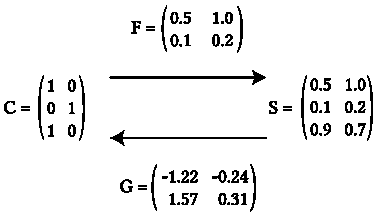
\includegraphics[width=200pt]{figures/fig3.1.pdf}
    \caption{Illustration of mapping between $C$ and $S$ matrix via $F$ (i.e. comprehension), and $S$ and $C$ matrix via $G$ (i.e. production). Note: In production, $C$ is referred to as $T$.}
    \label{fig:3_1}
\end{figure}
